%%%%%%%%%%%%%%%%%%%% author.tex %%%%%%%%%%%%%%%%%%%%%%%%%%%%%%%%%%%
%
% sample root file for your "contribution" to a contributed volume
%
% Use this file as a template for your own input.
%
%%%%%%%%%%%%%%%% Springer %%%%%%%%%%%%%%%%%%%%%%%%%%%%%%%%%%

% RECOMMENDED %%%%%%%%%%%%%%%%%%%%%%%%%%%%%%%%%%%%%%%%%%%%%%%%%%%
\documentclass[graybox]{svmult}

% choose options for [] as required from the list
% in the Reference Guide

\usepackage{mathptmx}       % selects Times Roman as basic font
\usepackage{helvet}         % selects Helvetica as sans-serif font
\usepackage{courier}        % selects Courier as typewriter font
\usepackage{type1cm}        % activate if the above 3 fonts are
                            % not available on your system
%
\usepackage{makeidx}         % allows index generation
\usepackage{graphicx}        % standard LaTeX graphics tool
                             % when including figure files
\usepackage{multicol}        % used for the two-column index
\usepackage[bottom]{footmisc}% places footnotes at page bottom

%\PassOptionsToPackage{hyphens}{url}
%\usepackage{fullpage}
\usepackage{url}
\usepackage{hyperref}
\usepackage{doi}
%\usepackage{natbib}
\usepackage{amssymb}
\usepackage{epstopdf}
\usepackage{wrapfig}
%\DeclareGraphicsRule{.tif}{png}{.png}{`convert #1 `dirname #1`/`basename #1 .tif`.png}

% see the list of further useful packages
% in the Reference Guide

\makeindex             % used for the subject index
                       % please use the style svind.ist with
                       % your makeindex program
\newcommand{\putabstract}{ Musical performances with touch-screen
  devices can be recorded by capturing a log of touch interactions.
  This new-media object can serve as an archive or as a basis for
  other representations of the musical work. This paper presents a
  protocol for logging touch-interactions as well as visualisations
  and gesture-scores generated from logs of a series of improvised
  ensemble performances on iPads. These objects record the
  performances for posterity and also allow deeper analysis of musical
  interactions present. }
%%%%%%%%%%%%%%%%%%%%%%%%%%%%%%%%%%%%%%%%%%%%%%%%%%%%%%%%%%%%%%%%%%%%%%%%%%%%%%%%%%%%%%%%%

\begin{document}

\title*{A Percussion-Focussed Approach to Preserving Musical Performance on Touch-Screens}
% Use \titlerunning{Short Title} for an abbreviated version of
% your contribution title if the original one is too long
\author{Charles Martin and Henry Gardner}
% Use \authorrunning{Short Title} for an abbreviated version of
% your contribution title if the original one is too long
\institute{Charles Martin \at Research School of Computer Science, The
  Australian National University, Canberra,
  \email{charles.martin@anu.edu.au} \and 
  Henry Gardner \at
  Research School of Computer Science, The Australian National
  University, Canberra, \email{henry.gardner@anu.edu.au}}

\maketitle
\abstract*{\putabstract}
\abstract{\putabstract}

\section{Introduction}

As an artistic experience, musical performance is fleetingly temporal
and the history of music abounds with technologies and traditions to
grab hold of musical performances, recording them in some format to be
archived, understood, and developed. All of our traditions of musical
recording, from rote-learning and notation, to the phonograph and
digital recording, have contributed to the ability of performers to
create new musical works and to the place of music in our cultural
landscape.

While western classial music is often defined by the score, and
popular music by the song or the recorded version, the practice of
free improvisation often defies the identification of a canonical
``musical work''. In free-improvised ensemble music, all decisions
about the notes to play are made in the moment by individual musicians
with the work ending only when all performers have stopped playing.
With each performance equally identifiable as a different work, the
output of free-improvisation ensembles is often represented only as
audio recordings with documented changes in personnel or
instrumentation the main indicator of difference between works. When
performing with computer-based instruments, however, musicians have
the opportunity to record the musical work in an extremely detailed
form by capturing a log of their interactions as well as audio or
video recordings.

In this chapter, we present a protocol for automatically documenting
free-improvised musical performances made on touch-screen computers.
Our protocol, and the touch-screen instruments with which it is used,
are designed from a percussionist-centred perspective. Rather than
particular notes and rhythms, the focus of traditional musical
notation, our protocol records detailed touch movements in absolute
time and abstract touch gestures identified during the performance by our
computer software. Given that ensemble interactions are one of the
most interesting aspects of free-improvised music, our protocol is designed
to connect to multiple touch-screen devices engaged in ensemble
performance over a local network or the internet.

We argue that this protocol can serve as an archival format that
addresses many of the issues with curating improvised music for the
specific case of performances on touch-screens. Not only does it allow
a much more comprehensive documentation of the performances, but it
allows these performances to be characterised, analyised, and
appraised through statistics calculated on the touch and gestural data
which is abstracted from the particular instruments used or the
musicians who played them. We also show how logs of touch-screen
performances can become new media art objects in their own right,
forming a basis for other representations of the improvised musical
work such as visualisations or scores.

We will describe our protocol for capturing touch interactions and how
it has developed from previous schemes for capturing and controlling
musical performances. We will also present the statistics and
visualisation tools used for analysing and comparing performances
documented with our protocol. Our protocol and these tools were
developed as part of a series of research projects in touch-screen
musical performance and we will discuss how they have influenced the
research and artistic outcomes of these projects. In particular, we
will discuss the experiences of using these systems with Ensemble
Metatone, a free-improvisation percussion group that participated in a
longitudinal study over eighteen months performing with our
touch-screen instruments.

% Although this protocol was developed for research purposes,
% visualisations and analyses generated from logged data has formed an
% important archive of the group's performances of \emph{MetaLonsdale}
% for four iPads

\footnote{\label{note1}The video recording, touch-interaction log,
  visualisation and score of a performance of \emph{MetaLonsdale} is
  available online:
  \url{http://charlesmartin.com.au/blog/2014/1/17/metalonsdale-for-four-ipads}.}

\section{Percussive Improvisation on touch-screens}

\subsection{Percussive Interaction}

Percussionists are unique among western classical instrumentalists in
that their artistic practice is defined by an approach to interaction
rather than by the instrument that they use. Percussionists perform by
``striking, scraping, brushing, rubbing, whacking, or crashing any...
available object''~\cite{Schick:2006fk}. Blades~\cite{Blades:1992kx}
discusses the earliest percussion instruments, idiophones, where the
body of an instrument creates the sound, rather than an air column or
string. He divides them by their method of interaction: ``shaken'',
``stamping'' (played with the hands or feet), ``scraped'',
``concussion'' (two parts struck together), and ``struck'' (with a
stick or non-sounding implement). These descriptions match taxonomies
of modern instruments (such as Cook~\cite{Cook:1997vn}) and focus on
the mode of interaction for the instruments rather than their physical
design.

Modern percussionists are accustomed to exploring non-traditional
objects to create music and use these percussive gestures to coax wide
varieties of timbres and musical gestures from simple instruments.
Performers of Xenakis' \emph{Psappha}~\cite{Xenakis:1975uq} or
Feldman's \emph{King of Denmark}~\cite{Feldman:1965uq} must design
their own multi-instrument setup to fit the composer's specifications.
To meet the requirement for metal instruments, for example, a
performer might find a car's suspension spring, a saw-blade or create
a unique object from scratch.

For percussionists, free improvisation is often a process of gestural
exploration, discovering new sounds from traditional and
non-traditional instruments and responding to other sounds in an
ensemble. Like some of the instruments in a modern percussion
ensemble, touch-screen computing devices can be struck, scraped and
rubbed with fingers and hands. Their percussive affordances, their
power to generate computer music and their widespread popularity,
motivate an exploration of the use of touch-screen devices in a modern
percussion ensemble.

\subsection{Composing with Gestures}

While traditional musical notation specifies sonic outcomes - pitch,
articulation and rhythm - it is possible to compose music by
specifying gestures used for interacting with instruments. For
percussionists, where gestures are transported across a variety of
instruments, this is a popular way of notating music for particularly
unconventional instruments. Thierry de May's famous work \emph{Music
de Tables}~\cite{May:1987fk} is written for three percussionists who
perform on the surfaces of regular tables. de May defines a vocabulary
of notation for gestures that are used with standard rhythmic notation
in the score. Burtner's \emph{Syntax of Snow}~\cite{Burtner:2011fk}
asks the solo performer to play a glockenspiel with one hand and a
bowl of snow with the other. The score sets out a complex scheme of
gestures for ``playing'' the snow, with a pair of symbols (see Figure
\ref{fig:SyntaxOfSnow}) for each gesture, representing the type of
gesture as well as hand position in the bowl.

\begin{figure}[h] \centering
\includegraphics[width=0.7\columnwidth]{figures/syntaxofsnow-excerpt.jpg}
\caption{An excerpt from Matthew Burtner's \emph{Syntax of
    Snow}~\cite{Burtner:2011fk} for solo glockenspiel and bowl of
  amplified snow. The composer defines a vocabulary of
  gestures for interacting with the snow with one hand represented by
  symbols below a regular staff for notes on the glockenspiel.}
\label{fig:SyntaxOfSnow}
\end{figure}

\subsection{Free-Improvised Performance}

Prolific Swedish improvisor Harald Stenstr\"om defined free-improvised
performance as the performance of music ``without any restrictions
regarding style or genre and without having predetermined what is to
be played''~\cite{Stenstrom:2009xy}. In the context of this project,
free-improvised ensemble performance is not only the chosen mode for
developing artistic works but a methodology for researching new
interactions with the iPad-based instruments. Bill Cahn, member of the
legendary percussion group, Nexus, writes that improvisation
encourages ``a deeper knowledge of the instruments and their
sound-making possibilities''~\cite{Cahn:2005uq}. Digital media
theorist Aden Evens writes that when improvising with an unfamiliar
instrument ``the musician generates novel and surprising results even
when applying familiar technique.''~\cite{Evens:2005kx}

Even though free-improvised performances have no score it can still be
useful to produce some kind of description of performances in order to
evaluate and critique this musical process. Stenstr\"om proposes a
terminology for free ensemble improvisation, including concepts such
as ``transitions'' between musical ideas and ``attractors'' such as a
steady pulse that encourage similar playing from other
performers~\cite{Stenstrom:2009xy}. It is hoped that this thesis will
produce a system for automated transcription of improvised
performances based on touch gesture, allowing more straightforward
evaluation and understanding of this kind of performance.

\section{Curating the Improvised}

\subsection{Representing the Musical Work}

\begin{figure}
  \centering
  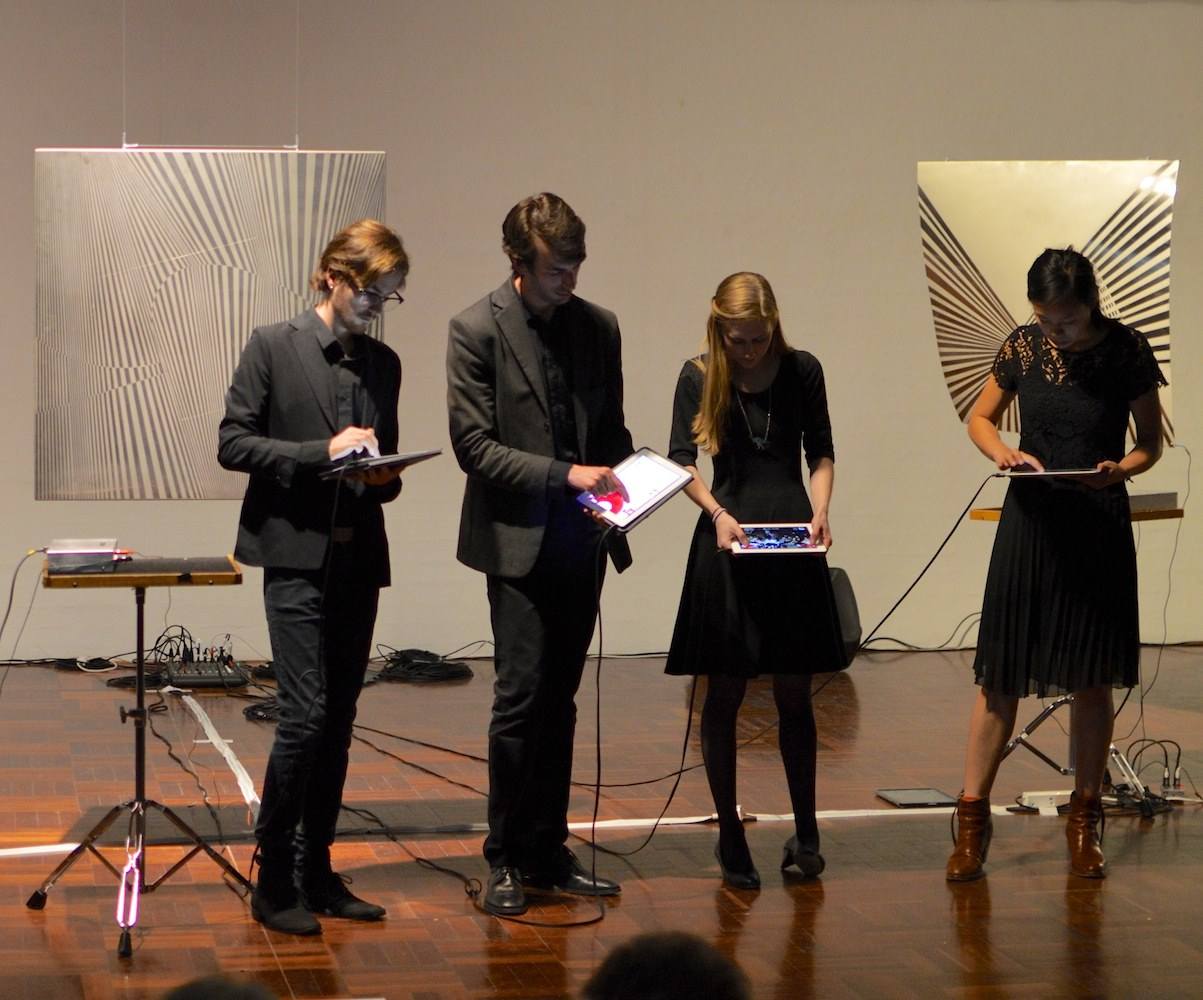
\includegraphics[width=\textwidth]{figures/ensemblemetatone}
  \caption{Ensemble Metatone performing \emph{MetaLonsdale} at the ANU
    School of Art Gallery in October 2013 (left to right: Jonathan
    Griffiths, Charles Martin, Christina Hopgood, Yvonne Lam).}
  \label{ensemblemetatoneperforming}
\end{figure}

It is widely recognised that musical works as well as new media
artefacts can have a number of interacting
representations~\cite{Rinehart:2007pi}. Musical works might be
directed by a score; be ``thick'' or ``thin'' depending on the the
freedom of interpretation afforded the performers; be represented in
live performance, studio recordings, or by computer generated
renderings; and may be composed or improvised~\cite{Davies:2005fj}.
Combinations of these representations are often collected together
form an archive of a musical work.

Free improvised music, where performers do not follow a set musical
structure, is usually preserved using only audio and video recordings.
While the improvised solos of famous jazz musicians are often
transcribed, this is extremely uncommon for free-improvised ensemble
performances. For improvised music on touch-screens, a log of
touch-interactions captured by the performance suplements traditional
recordings and could take the place of a ``score'' in documenting such
performances. While scores are generally used for composition, their
use as documentation for new media artworks has been
acknowledged~\cite{MacDonald:2009ve}. Such a log would also satisfy
Manovich's principles for a new media artwork~\cite{Manovich:2002ly}.
In particular, the log of touch-interactions is variable, forming the
basis for derivative artworks that also represent aspects of the
original performance.

Free-improvisation is often a process of gestural exploration,
discovering new sounds and responding to other sounds in an ensemble.
In audio recordings of these performances, the sonic result of the
gesture is captured but the gesture itself lost. While the gestural
component of musical performance may not be as integral as in dance or
other physical performance, it still contributes to the audience's
perception of a work and represents a certain amount of the
performers' intention. Although touch-interaction data is not a
complete record of performers' gestures it is simple to obtain and
easily transformed into other representations of a performance.



% - percussion interaction - more details
% - composing with gestures - more details (e.g. from TPR 2013.
% - comparison to TUIO: \cite{TUIO_KBBC05}


% \subsection{Composing with Gestures}

% While traditional musical notation specifies sonic outcomes - pitch,
% articulation and rhythm - it is possible to compose music by
% specifying gestures used for interacting with instruments. For
% percussionists, where gestures are transported across a variety of
% instruments, this is a popular way of notating music for particularly
% unconventional instruments. Thierry de May's famous work \emph{Music
% de Tables}~\cite{May:1987fk} is written for three percussionists who
% perform on the surfaces of regular tables. de May defines a vocabulary
% of notation for gestures that are used with standard rhythmic notation
% in the score. Burtner's \emph{Syntax of Snow}~\cite{Burtner:2011fk}
% asks the solo performer to play a glockenspiel with one hand and a
% bowl of snow with the other. The score sets out a complex scheme of
% gestures for ``playing'' the snow, with a pair of symbols (see Figure
% \ref{fig:SyntaxOfSnow}) for each gesture, representing the type of
% gesture as well as hand position in the bowl.

% \begin{figure}[h] \centering
% \includegraphics[width=0.7\columnwidth]{syntaxofsnow-excerpt}
% \caption{An excerpt from Burtner's \emph{Syntax of Snow}.}
% \label{fig:SyntaxOfSnow}
% \end{figure}

\section{Ensemble Metatone and MetaLonsdale}

Ensemble Metatone was brought together to study the process of
performing free-improvised music on specially designed iPad apps and
percussion instruments in Canberra, Australia. The members of the
group (including one of the authors of this paper) are all trained in
classical percussion with experience as improvisors.

Over a series of studio rehearsals, the group worked with the
``MetaLonsdale'' app to develop a work which was performed at
festivals and events throughout 2013. The studio rehearsals and a
public recital were recorded with seperate tracks of audio for each
iPad, multiple camera angles, and a log of touch-interactions.

The app used a percussion-inspired interaction scheme allowing
performers to access pitched percussion sounds and field recordings.
Most of the iPad screen was a performance surface with few graphical
UI elements. Tapping the screen produced short sounds at a pitch
determined by the location of the tap. Swiping played continuous field
recordings with volume controlled by the velocity of the swipe. The
app featured two UI switches that controlled simple delay functions,
that repeat tapped notes, and switchable auto-play features, that
alogrithmically produced background sounds. A button on both apps
allowed the performer to shuffle the available sounds.

\begin{figure}
  \centering
  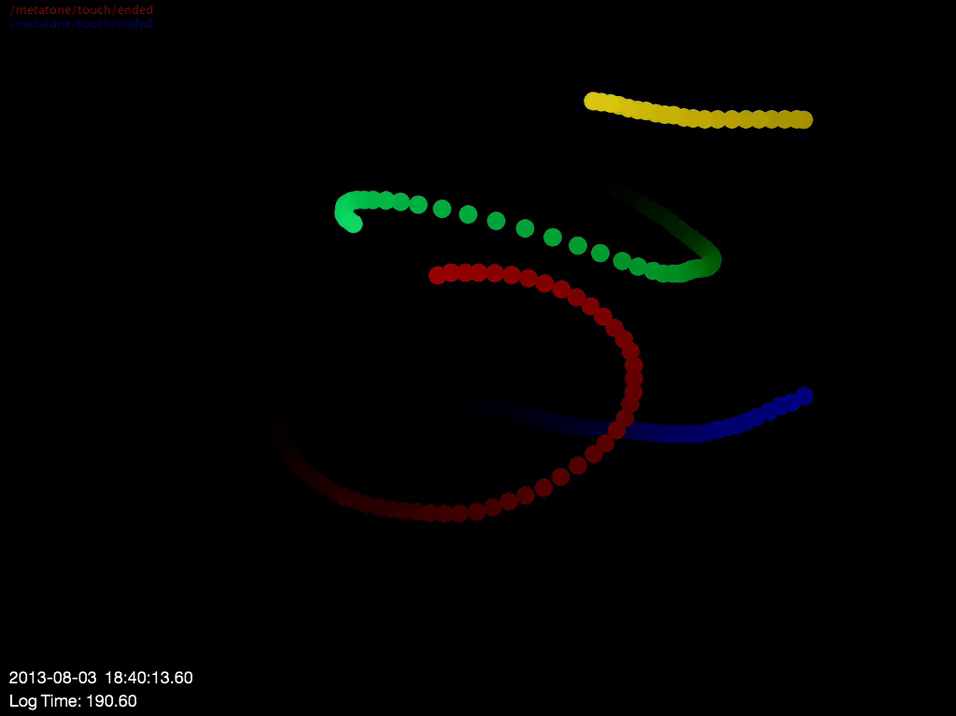
\includegraphics[width=\textwidth]{figures/metatoneanimation1}
  \label{metatoneanimation1}
\end{figure}
\begin{figure}
  \centering
  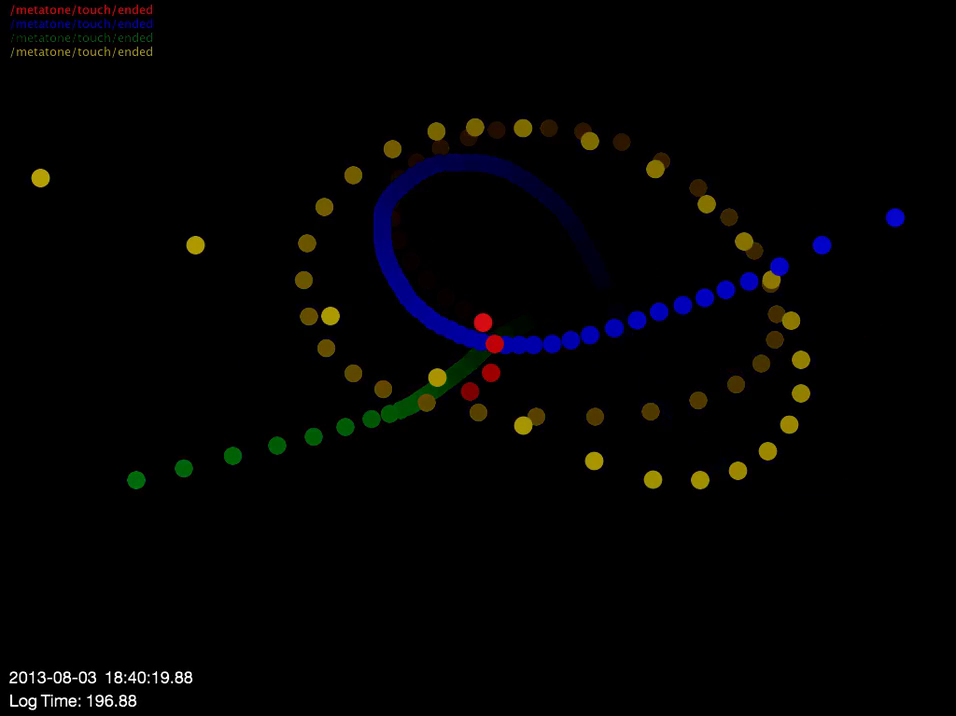
\includegraphics[width=\textwidth]{figures/metatoneanimation3}
  \label{metatoneanimation2}
\end{figure}
\begin{figure}
  \centering
  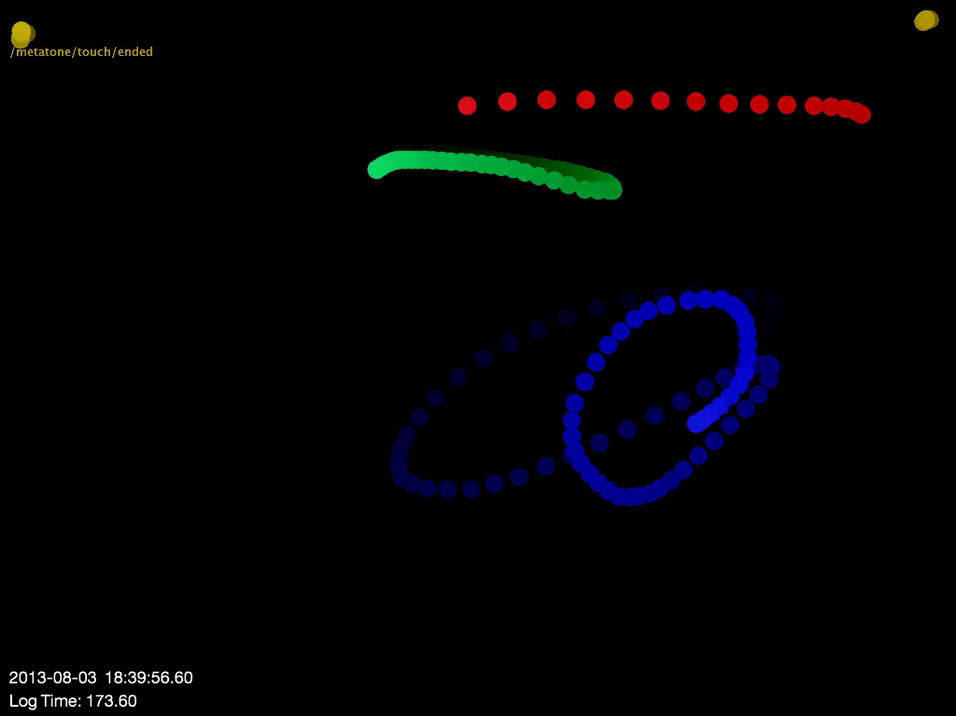
\includegraphics[width=\textwidth]{figures/metatoneanimation2}
   \caption{Stills from an animation of an Ensemble Metatone
     performance. The full animation can be viewed online\footref{note1}.}
  \label{metatoneanimation3}
\end{figure}

\section{Protocols for musical touch interaction}

In performances with our iPad apps, all touch interactions during the
performance are transmitted over a Wi-Fi network to server software
running on a laptop or a remote virtual server. We have developed a
relatively simple protocol for formatting touch and other interaction
data using the OSC~\cite{osc-nime2009} (Open Sound Control) standard.
The data is transmitted either through Unix sockets using the UDP
protocol (as is typical for OSC messages) or through
WebSockets~\cite{Fette:2011eu}, which is the preferred method due to
increased reliability of transmission and the ability to easily open a
bi-directional connection with a remote server. 

\subsection{Protocols for capturing performance data}

Musical data has been abstracted from the temporality of performance
for centuries since the development of musical notation. Mechanical
instruments such as music boxes and barrel organs developed in the
18th century~\cite{Fowler:1967kq} first allowed music to be
``programmed'' rather than performed. More refined mechanical
instruments such as the ``reproducing piano'', which appeared at the
turn of the 20th century~\cite{Kapur:2005fk}, allowed a musician's performance to be
automatically transcribed and converted into a paper ``piano roll''
that could be re-played many times. All of these technologies have had
an impact in the study of music as well as it's performance. Musical
notation enabled the field of musicology, where the musical score has
traditionally been priveleged as the canonical representation of a
musical work. The piano-roll performances of many famous pianists were
made before audio recording was available or widespread and have been
used to analyse their performance styles.

An important antecedent of our work was the
MIDI~\cite{midi1996complete} (Musical Instrument Digital Interface)
protocol, which was developed in the late 1970s to connect electronic
music \emph{controllers}, such electronic versions of keyboards, drums
and wind instruments and new musical interfaces such as ``THE
HANDS''~\cite{TheHandsArticle}, with electronic synthesisers or
digital recording systems. While this standard was intended as a
control interface for live performance or recording, it was subverted
by digital artists and researchers who recognised that the MIDI trace
of a musical performance could be used for other purposes. While MIDI
was originally designed to be used with a physical serial connection,
virtual MIDI connections are commonly used to connect multiple pieces
of software on one computer system and a networked version of MIDI
also exists\cite{Lazzaro:2004pb}.

While the success of MIDI is ongoing, the semantics of the protocol is
mostly restricted to note and keyboard perspective on musical data.
The typical MIDI interactions are ``note on'' and ``note off''
messages, each of which contain a pitch and dynamic (volume) value.
Changing parameters while a note is playing can be achieved by
simultaneously sending one of a limited number of ``continuous control'' messages while the
``note on'' is held. In an effort to develop a semantics-free format
for musical control that better reflected the needs of modern computer
systems, OSC~\cite{osc-nime2009} (Open Sound Control) was provide a
standard message format but with the specific content of the messages
up to the application developer. This flexibility has contributed to
the success of OSC not just in computer music, but in professional
applications such as show control although it is not common in
commercial electronic instruments. 

Some have attempted to define protocols using OSC to standardise
interaction with certain types of interface. TUIO~\cite{TUIO_KBBC05}
is one such protocol designed for table interfaces that were used with
touch or special objects, ``fiducial markers'', that could be tracked. 

% - MIDI
% - TUIO
% - OSC
% - other formats?


\subsection{The Metatone Log Format}


Touch interactions were transmitted as OSC messages over a Wi-Fi
network from the four iPads to a laptop. Messages from touches in the
performance area were sent with the location of the touch and
velocity. Touch-down events were denoted with a velocity of zero while
touch-ended events were represented with a different OSC address.
Messages were also sent when the button was pressed or a switch was
moved in the UI. A logging application on the laptop assigned
timestamps to each message and wrote it to a text file for later
analysis.

This scheme for logging touch-interactions (see table \ref{oscschema})
was chosen to study the process of improvising with iPad instruments
and not necessarily for replaying performances. It does not capture
other touch ``state'' variables such as a unique identifier for each
touch. It also does not attempt to keep track of OSC messages that
might be delayed or lost, or network communications that took place
between the iPads. However, the log is extremely useful as a recording
of interaction with the instruments and can be transformed into other
representations of the performance. While the logs were created for
research purposes they also serve as representative artefacts of the
performance along with the audio and video recordings.

\begin{table}
  \begin{tabular}{|l|l|}
  \hline
  OSC Address           & Parameters \\ \hline
  /metatone/online      & device  \\     
  /metatone/touch       & device, X, Y, velocity \\
  /metatone/touch/ended & device \\  
  /metatone/switch      & device, switch, position\\ \hline
  \end{tabular}
  \caption{Scheme for OSC messages from the Metatone iPad apps. The
    switch message was also used to record presses of the UI button in
    the app.}
  \label{oscschema} 
\end{table}

\subsection{Animations}

To understand the structure of the improvised performances we wanted a
visual representation of the performers' touch gestures to watch
alongside the audio and video recordings of each performance. A
Processing sketch was produced that read the captured log files and
rendered an animation of all four players' touches in the space of one
iPad screen with different players distinguished by colour. The sketch
also draws a date and time stamp on each frame as well as text
notifications of switch and button messages.

The resulting animations presents an entirely new view of the
performance which was not visible to the performers or audience on the
day. As all the touch movements are layered in one performance area it
is immediately clear when performers mimic each other, form sections,
or experiment with a new musical idea. From the researcher's point of
view, the animation also gives a ``performer's perspective'' on touch
interaction, allowing us to connect patterns of touches with musical
gestures that the performers discuss after rehearsals.

\subsection{Tracking Gestures as a Score}

Interpreting the gestures of musicians improvising on touch-screen
instruments was a research goal of working with Ensemble Metatone. One
approach to this has been the application of machine-learning
algorithms to logs of touch-interaction. After the initial rehearsal
series took place, a vocabulary of touch gestures was developed from
qualitative analysis of the rehearsals and discussions among the
performers. From this vocabulary, examples of each gesture were
recorded and the resulting log used to train a Random Forest
Classifier algorithm~\cite{Breiman:2001kx}. Five second windows in the
logs are used to calculate feature vectors which are classified by the
algorithm. While research into how this technique can be applied in
live performance is ongoing, the classifier is able to produce an
interpretation of recorded performances as a ``score'' of gestures. In
figure \ref{gesturescore}, each performer's gesture is given by the
coloured lines which can move between the nine possible gestures in
the vocabulary. Graphical scores like figure \ref{gesturescore} are
common in contemporary music and the representation of a performance
as a sequence of gestures recalls descriptions of free-improvised
music as ``transitions'' and ``attractors''~\cite{Stenstrom:2009xy}.

\begin{figure}
\centering
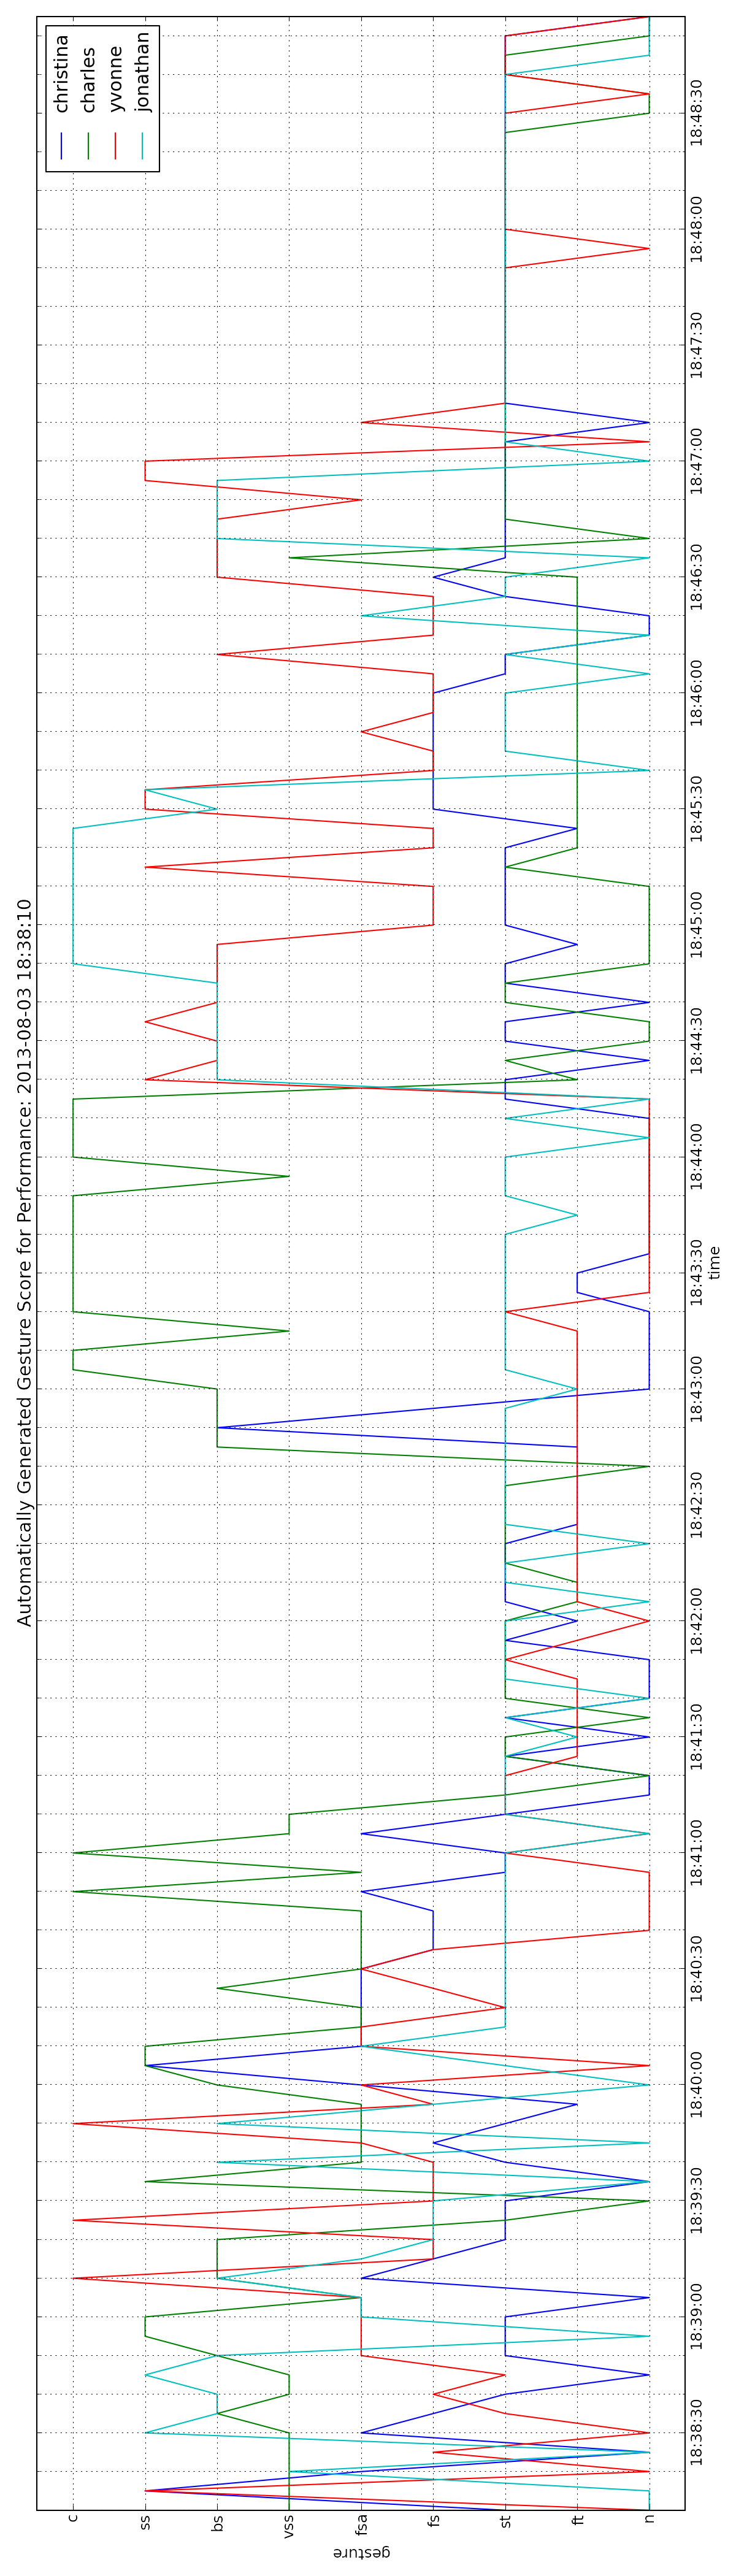
\includegraphics[height=0.9\textheight]{figures/score20130803vert}
\caption{An automatically generated ``gesture score'' for the
  \emph{MetaLonsdale} performance on 3-8-2013. }
\label{gesturescore}
\end{figure}

The scores produced so far are already helpful in understanding at a
glance the overall flow of a performance. In this way they may be more
useful archival documents of a performance than, for example, a still
photograph of the stage setup.

\section{Conclusions}

By logging touch-interactions in Ensemble Metatone's performances on
iPads we recorded aspects of the musical work that are not accessible
in traditional archives of free-improvised music. The logs also allow
further insight into the gestural nature of performance on
touch-screens. In particular, animations of the performers' touches
aided the development of a vocabulary of gestures.  Graphical
``gesture scores'' following this vocabulary were generated from
the logs automatically using a Machine-Learning algorithm. 

These alternative representations have allowed a more comprehensive archive
of performances and one that affords more insight into the performers'
gestural and musical intent and ensemble interactions as well as
their sonic output. As more performances are logged, it is hoped that
these representations will allow us to track the group's musical
developments or different approaches taken with future touch
instruments. The representations could also be used in performance as
visual accompaniments for the audience or displayed to the players as
real-time feedback.

\bibliographystyle{spphys}
\bibliography{2013ComputerMusic}
\end{document}

% %
% \section*{Appendix}
% \addcontentsline{toc}{section}{Appendix}
% %
% %
% When placed at the end of a chapter or contribution (as opposed to at the end of the book), the numbering of tables, figures, and equations in the appendix section continues on from that in the main text. Hence please \textit{do not} use the \verb|appendix| command when writing an appendix at the end of your chapter or contribution. If there is only one the appendix is designated ``Appendix'', or ``Appendix 1'', or ``Appendix 2'', etc. if there is more than one.